\documentclass{article}
\usepackage{graphicx}
\usepackage{latexsym}
\usepackage[french]{babel}
\usepackage[utf8]{inputenc}
\usepackage[T1]{fontenc}
\usepackage{listings}

\title{Rapport du projet C++ : Lancer de rayons}
\author{Mathieu \textsc{Mari} \and Xavier \textsc{Montillet}}

\begin{document}

\title
\tableofcontents
	

\section{Introduction}
Dans ce nouveau projet, nous nous sommes intéressé à la technique du lancer de rayons et nous l'avons implémenter en C++.
Cette technique permet de générer des images 3D à partir de la déscription des objets présent dans la scène ainsi que de la position de la caméra. Elle a son utilité dans les logiciels d'images de synthèse, la création de jeux vidéos, la simulation numérique\dots  	

\section{Implémentation en C++}
	\subsection{Principe général}
	\paragraph{}		
Afin de générer l'image 3D d'une scène, il faut deja définir quels sont les objets qui composent la scène, c'est dire définir quel est leur type (sphère, plan, \dots), quelle est leur position, leur couleur, leur texture\dots. Ensuite, il faut choisir la posistion des sources lumineuses puis leur couleur, leur intensité\dots Enfin, il faut positionner la caméra qui observe la scène. Pour cela, on choisit un point qui sera la position de l'objectif, puis la position de l'ecran sur lequel l'image sera projetée.

	\paragraph{}
		Fabriquer une image, c'est calculer pour chaque pixel sa couleur. Dans cette optique, le principe de la technique du lancer de rayons consiste à créer une demi-droite ayant pour origine l'objectif de la caméra et passant par le un pixel de l'écran. On regarde quel objet de la scène est intersecté en premier par la demi-droite. On calcule ensuite la couleur du pixel en regardant combien de sources éclairent le point d'intersection entre la demi-droite et l'objet, quel est la couleur de l'objet et des sources, est-ce qu'il y a reflection, refraction, transparence\dots

		\subsection{Les différentes classes utilisées}

Afin de représenter les différents éléments qui seront nécessaires à la technique du lancer de rayons et leur dépendance mutuelle, nous allons utiliser les classes C++.

\subsubsection{Dépendances des classes}
Le schéma de dépendance des classes est le suivant :
	\begin{center}
    		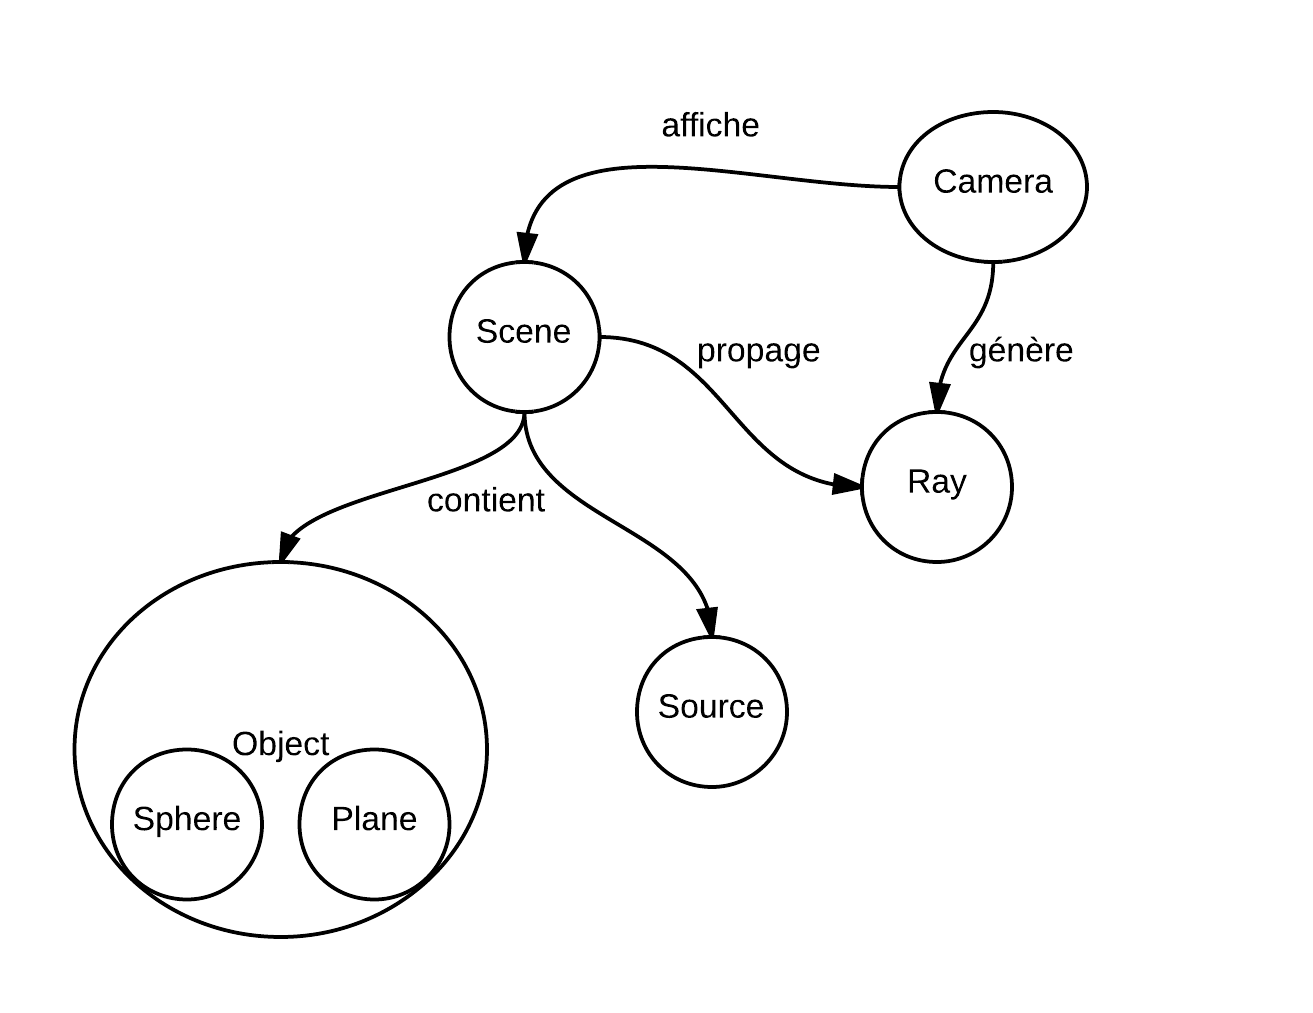
\includegraphics[height = 7cm]{schema.png}
  		\end{center}

	\begin{itemize}
\item La classe \emph{Scene} est la classe principale. Elle contient des objets de la classe \emph{Object} qui contient elle-même deux sous-classes : \emph{Sphere} et \emph{Plane}. 
\item La classe \emph{Scene} contient également des sources lumineuses de la classe \emph{Source}.
\item La caméra, représentée par la classe \emph{Camera} est indépendante de la classe \emph{Scene} car il nous semblait raisonnable que la caméra soit indépendante le la scène. En effet, la scène n'a pas besoin de savoir où se situe la caméra : c'est la caméra qui observe la scène! 

\end{itemize}
Toutes ces classes interfèrent entre elles grâce à des rayons de la classe \emph{Ray} : la caméra fabrique des rayons qui vont se propager dans la scène. 



D'autres classes nous sont utiles dans la réalisation de l'algorithme de lancer de rayons.

\subsubsection{La classe \emph{Light}}
Cette classe permet de représenter un rayon lumineux. Elle possède trois attributs : une composante \emph{red}, une composante \emph{green}, et une composante \emph{blue}.
La différence avec la classe \emph{Color} est que les composantes ne sont pas comprisent entre $0$ et $255$ mais entre $0$ et $+\infty$.
Ceci permet de représenter de façon implicite l'intensité d'une lumière, (on peut imaginer prendre le max des composante par exemple). Ceci permet d'additionner des lumières en additionnant simplement composante par composante, sans avoir à se préocuper de faire un barycentre avec différents coefficients. 


Nous avons codé une fonction permettant de transformer une lumière en une couleur (l'image renvoyée à la fin ne connait que des couleurs ayant des composantes comprises entre $0$ et $255$. Pour cela nous composons les composantes par la fonction $x \rightarrow 255\tanh(x)$. 

\subsubsection{La classe \emph{Texture}}
	La couleur d'un pixel dépend de la texture de l'objet visé. En effet, l'effet visuel ne sera pas le même suivant si l'objet est brillant, mate, transparent\dots La classe \emph{Texture} permet donc de représenter ces différentes caractéristiques. Cette classe est essentielle si nous ne voulons pas à chaque fois redéfinir les méthodes de la classe \emph{Object}. 

\subsubsection{Les classes auxiliaires}
	\begin{description}
		\item[La classe \emph{Point} : ]
Cette classe permet de distinguer un vecteur d'un point. Même si on peut représenter un point par un vecteur, il n'est pas très correct d'additionner deux points par exemple. Nous définissons donc des fonctions definissant les opérations entre la classe \emph{Point} et la classe \emph{vector}.

		\item[La classe \emph{Option} : ]
	\end{description}
  
\section{Comment renvoyer la couleur d'un pixel ?}
Afin de générer l'image finale, la caméra envoie pour chaque pixel un rayon (de la classe \emph{Ray}) partant de l'objectif et passant par le pixel correspondant. Les programmes que nous avons codé consistent à associer à chacun de ces rayons une couleur.

\subsection{Première étape : Trouver le premier objet de la scène intersécté par le rayon}
Afin de touver le premier objet de la scène intersecté par le rayon, nous calculons pour chaque objet si le rayon l'intersecte puis parmi tous les objets intersectés nous prenons l'objet le plus proche de la caméra. Dans un deuxième temps nous renvoyons le point $P$ (classe \emph{Point}) d'intersection entre le rayon et l'objet.

\subsection{Deuxième étape : Calcul de la couleur}
A présent, il faut savoir si le point $P$ est éclairé par les sources lumineuses. Pour cela pour chaque source $S$ de la scene, nous regardons si le rayon reliant $P$ à $S$ intersecte au moins un objet de la scène autre que l'objet courant. si l'objet est une sphère nous verifions également si le cosinus entre la normale au point $P$ et le vecteur $PS$ est positif (le contraire indiquerait que la source se situe de l'autre coté de la sphère).
Pour chaque composante ($r$ par exemple) nous calculons la lumière résultante par la formule : 
\begin{equation}
	$r_{final} = \sum_{s \in \{ \text{sources éclairant} P \}} r_s*\lambda(s)*\frac{r_{objet}}{255}$
\end{equation}
où $\lambda(s)$ est le cosinus entre la normale à l'objet en $P$ et le vecteur $PS$. 
On obtient ainsi une lumière que l'on transforme en couleur grâce à la fonction $\th$

Remarque : Cette première version de moteur de lancer de rayon ne tient compte que de l'aspect mâte des objets, on ne considère pas la reflection ni la transparence des objets.

\section{Ameliorations}

A partir du moteur de lancer de rayons que nous avons codé, nous pouvons penser à diverses améliorations.
\subsection{Amélioration visant à rendre l'image plus réaliste}
	\begin{itemize}
		\item Enrichir la classe \emph{Object} avec d'autres objets comme des objets définis par des équations cartésiennes par expemple.
		\item Rendre la classe Texture un peu plus exhaustive en prenant en compte la transparance, un coefficient de reflexivité, un indice de réfraction\dots
		\item Imaginer des objets ayant une texture non uniforme.
		\item Chercher à représenter des objets ayant une certaine épaisseur.
		\item Intégrer des phénomènes physiques tels que la diffraction, la réfraction\dots
	\end{itemize}

\subsection{Avancer vers un moteur plus fonctionnel\dots}
	\begin{itemize}
		\item Uiliser deux caméras, générer deux images que l'on filtre l'un avec du rouge et l'autre avec du bleu par exemple, et observer grâce à des lunettes, une image en trois dimensions.
		\item Rajouter une dépendance temporelle des objets et regarder la scène évoluer.
		\item Déplacer la caméra dans la scène et visualiser de façon "fluide" les transformations, dans le but de faire des vidéos de synthèse par exemple.
	\end{itemize}

\section{Conclusion}
Lors de ce projet sur la technique du lancer de rayons, nous avons compris à quelle point les classes peuvent s'avérer être des outils puissant lors de l'implémentation de problèmes de ce type. En effet, la multiplicité des éléments d'un moteur de lancer de rayon (scène, rayon, lumières, couleurs, objets, caméra, texture, etc) et leur forte intriquation mutuelle conduit à penser les programmes à travers les différentes dépendances des éléments entre eux et donc d'utiliser des classes. Ce projet à conduit à générer des images relativement réalistes, d'une scène contenant des sphères et des plans.
	


\end{document}
